\chapter{Teleportation}
\label{sec:8_teleportation}

%\begin{abstract}
% Hi, and welcome to Lesson 8 on "Teleportation".

Teleportation is one of the most wonderful and most fundamental protocols in quantum information processing. It is used extensively in quantum computation and quantum communication, so let's learn about it.
%\end{abstract}

\section{Introduction}
\label{sec:8-1_introduction}

% Step One: Introduction

How do we transmit information in a quantum network? Before we answer that let's see what happens classically. In Ch.~\ref{sec:1_Introduction}, we saw the example of the Great Wall of China. If a guard tower was under attack, they lit a fire to alert the other guard towers and ask for help. That message really was carried by the photons which originated from the fire and reached the other guard towers, where they entered the eyes of the other guards, who then were able to act. In modern times, if we want to download some data or we want to communicate over the classical Internet, the message is a bit string and again it is carried by photons in optical fibers. So in classical networks, when we transmit some message, we have to transmit the physical system itself  -- that is to say, the set of photons -- that is encoding the message.
\begin{figure}[H]
    \centering
    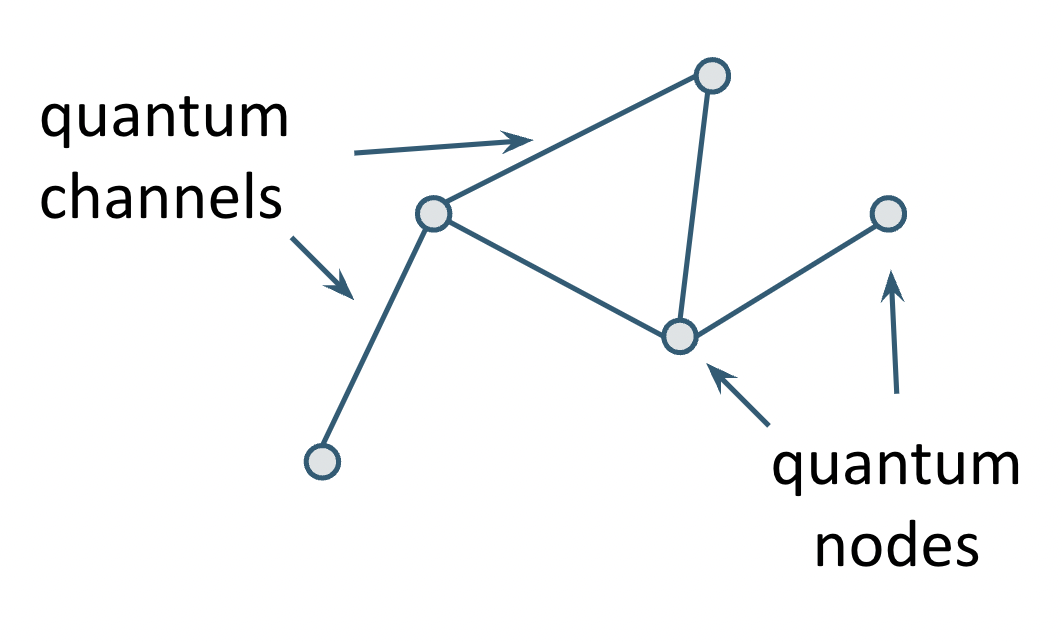
\includegraphics[width=0.8\textwidth]{lesson8/quantum-network.png}
        \caption{A quantum network consists of quantum nodes, and quantum channels that we will call links.}
    \label{fig:quantum-network}
\end{figure}
\begin{figure}[H]
    \centering
    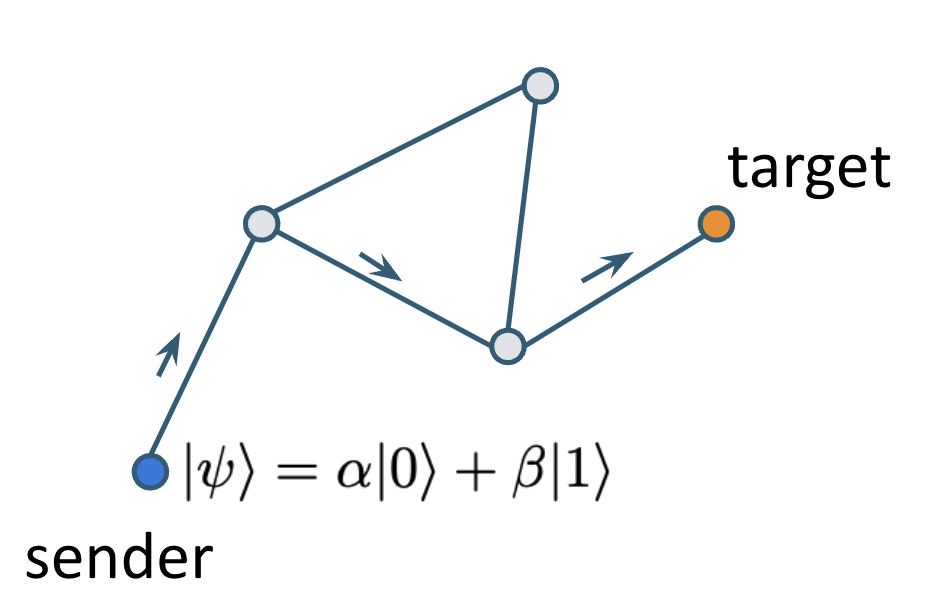
\includegraphics[width=0.8\textwidth]{lesson8/hop-by-hop.png}
        \caption{Physically moving a quantum message hop-by-hop through a network.}
    \label{fig:hop-by-hop}
\end{figure}
\begin{figure}[H]
    \centering
    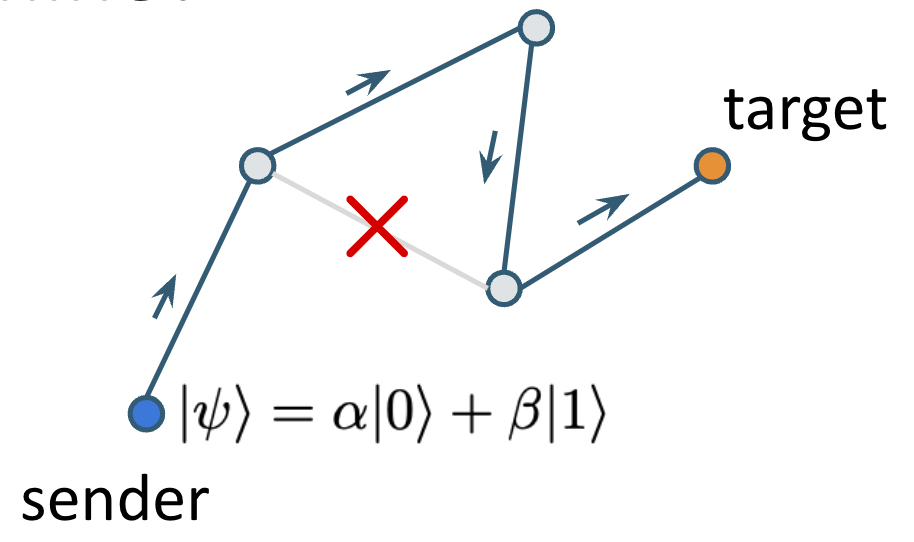
\includegraphics[width=0.8\textwidth]{lesson8/link-down.png}
        \caption{Rerouting when a link goes down.}
    \label{fig:link-down}
\end{figure}
\begin{figure}[H]
    \centering
    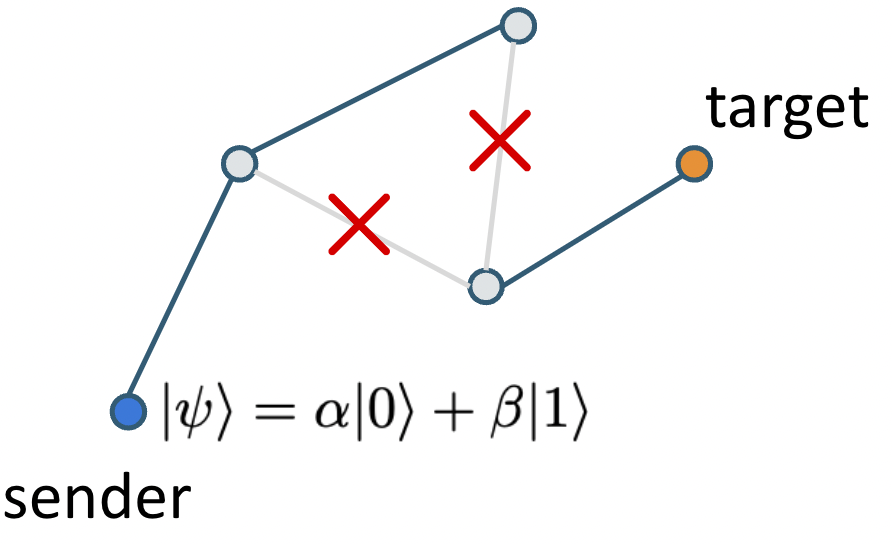
\includegraphics[width=0.8\textwidth]{lesson8/partitioned.png}
        \caption{A partitioned network.}
    \label{fig:partition}
\end{figure}


However in quantum physics, it's a little bit different. We can also transmit the (quantum) message without transmitting the (quantum) physical system. Consider a quantum network like Fig.~\ref{fig:quantum-network}, and let's say that we want to use the old-fashioned way of transmitting the message using a physical system that is encoding it. In this network, the circles represent our nodes and the lines represent the links, or quantum channels, between the nodes. The sender, represented by the blue node in the figure, is in possession of some pure state $\ket{\psi} = \alpha\ket{0}+\beta\ket{1}$, and  wants to send this state to the target given by the orange network node. As in Fig.~\ref{fig:hop-by-hop}, the sender can decide (or the network can decide) to send it first to its neighboring network node, then to the next network node, and then finally to reach the target. But what happens if one of the quantum links is not working? Well, in this particular case, it's not a big problem because the message can be simply rerouted to go around the damaged link and still reach the target. But what happens if another link is down? Well in this case, the quantum portion of our network is \emph{partitioned} and it seems like we cannot transmit the message to the target...unless we use teleportation! (Here, we assume that the supporting classical network remains intact, only the quantum channels are going up or down.) We can teleport this state from the sender to the target, provided that some initial conditions are met. We can move the information itself without moving the actual physical system. That physical system remains stationary.

\begin{figure}[H]
    \centering
    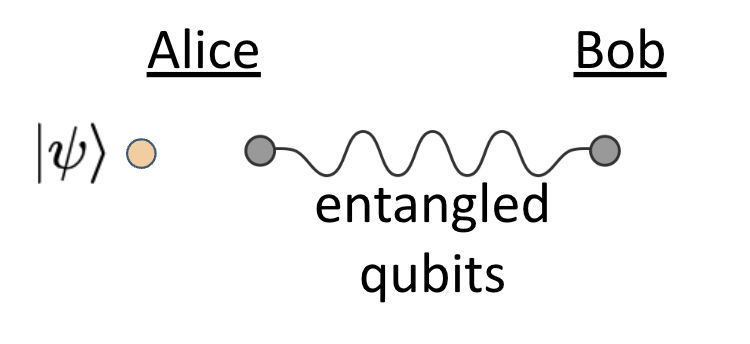
\includegraphics[width=0.8\textwidth]{lesson8/teleportation-setup.png}
        \caption{The setup for teleportation: Alice has the data qubit to be teleported, and Alice and Bob share a Bell pair.}
    \label{fig:teleportation-setup}
\end{figure}

\begin{figure}[H]
    \centering
    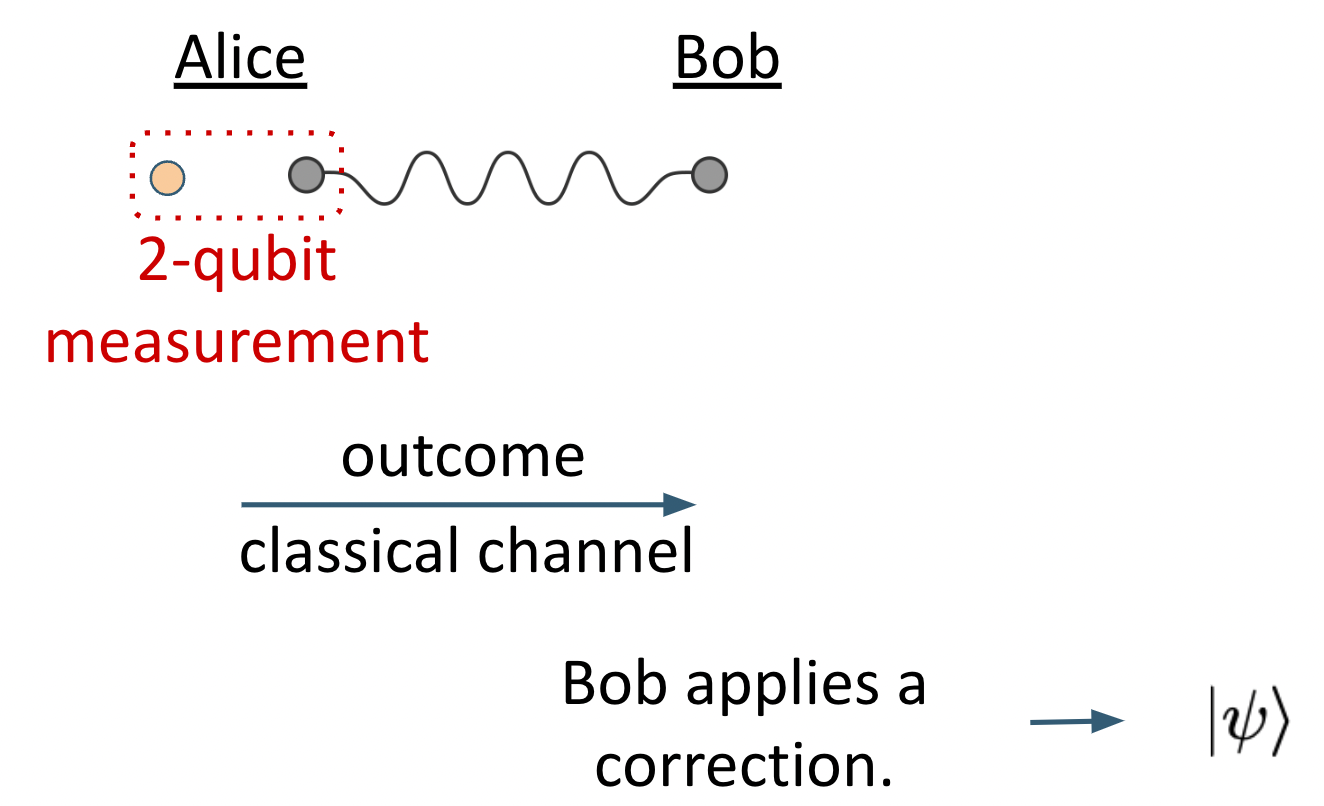
\includegraphics[width=0.8\textwidth]{lesson8/teleportation.png}
        \caption{Teleportation.}
    \label{fig:teleportation}
\end{figure}

This is the outline of the protocol: Call our sender "Alice", and she wants to send the quantum state $\ket{\psi}$ to her friend "Bob".  Alice and Bob start by sharing an entangled pair of qubits. Then Alice does a two-qubit measurement on both of her qubits. That measurement provides her with two classical bits, because the measurement is on two qubits.  Naturally, this means that there are four possible outcomes. Alice then communicates this outcome to Bob via a classical channel.  Bob then receives this classical message, applies some local corrections, and he ends up with the desired state $\ket{\psi}$. 

Now you see the two conditions necessary to maintain our ability to teleport quantum data even when the quantum network is partitioned: we must have a supply of entanglement, and we must have the ability to exchange classical messages.

\section{Teleportation protocol}
\label{sec:8-2_teleportation_protocol}

% Step Two: Teleportation Protocol

Let's look at the protocol in more mathematical detail.  First, consider the initial state in our protocol. Alice has an arbitrary qubit given by
\begin{align}
    \ket{\psi} = \alpha\ket{0} + \beta\ket{1}.
\end{align}
Alice and Bob also share an entangled state. It's one of the Bell states, $\ket{\Phi^+}$ (phi plus), which is equal superposition of zero zero and one one. In Fig.~\ref{fig:teleportation-setup}, we represent it as a wavy line. We label the qubits as follows: $A_1$ is the first qubit of Alice which is her state that she is trying to communicate to Bob. $A_2$ is her second qubit which is one part of the entangled Bell pair, and we designate Bob's qubit which is part of the entangled pair that he is sharing with Alice as $B$.

If we write out the initial state in its full form, we have
\begin{align}
    \begin{aligned}
|\psi\rangle_{A_{1}}\left|\Phi^{+}\right\rangle_{A_{2} B} &=(\alpha|0\rangle+\beta|1\rangle)_{A_{1}} \frac{1}{\sqrt{2}}(|00\rangle+|11\rangle)_{A_{2} B} \\
&=\frac{1}{\sqrt{2}}(\alpha|000\rangle+\alpha|011\rangle+\beta|100\rangle+\beta|111\rangle)_{A_{1} A_{2} B}.
\end{aligned}
\end{align}
$\ket{\psi}_{A_1}$ is Alice's input state that she wants to communicate, and the state $\ket{\Phi^+}$ spans qubits $A_2$ and $B$.
%We can write it out like this, and then expand to get the following superposition of basis states- (zero zero zero), (zero one one), (one zero zero), and (one one one), each with the corresponding probability amplitudes.

Then, Alice performs a two-qubit measurement. This is known as a \emph{Bell basis measurement} or just a \emph{Bell measurement}\index{Bell measurement}.
%So these are the following bell states- phi plus is given as a superposition of zero zero and one one. Phi minus is this similar superposition between (zero zero) (one one), but now we have a negative phase here. And psi plus is where the qubits are anti-correlated it's (zero one) plus (one zero), and psi minus is (zero one) minus (one zero). And 
Doing a measurement in the Bell basis is basically asking the question: which of the following states is Alice's state in? 
\begin{align}
    \begin{array}{ll}
\left|\Phi^{+}\right\rangle=\frac{1}{\sqrt{2}}(|00\rangle+|11\rangle) & \left|\Phi^{-}\right\rangle=\frac{1}{\sqrt{2}}(|00\rangle-|11\rangle) \\
\left|\Psi^{+}\right\rangle=\frac{1}{\sqrt{2}}(|01\rangle+|10\rangle) & \left|\Psi^{-}\right\rangle=\frac{1}{\sqrt{2}}(|01\rangle-|10\rangle)
\end{array}
\end{align}
To help us with answering that question, we have to rewrite our initial state in a slightly different form. To do that we will use the following trick: instead of writing the state using normal terms like $\ket{00}$ for the two qubits that Alice has, we can write it as a superposition of two of the Bell states using the following identities:
%, namely zero zero (you can check yourself can be written as superposition of phi plus and phi minus), zero one is then written as a superposition of psi plus and psi minus, and similarly the states one zero and one one can be written as superpositions but with negative phases over there.
\begin{align}
    \begin{array}{ll}
|00\rangle=\frac{1}{\sqrt{2}}\left(\left|\Phi^{+}\right\rangle+\left|\Phi^{-}\right\rangle\right) & |01\rangle=\frac{1}{\sqrt{2}}\left(\left|\Psi^{+}\right\rangle+\left|\Psi^{-}\right\rangle\right) \\
|10\rangle=\frac{1}{\sqrt{2}}\left(\left|\Psi^{+}\right\rangle-\left|\Psi^{-}\right\rangle\right) & |11\rangle=\frac{1}{\sqrt{2}}\left(\left|\Phi^{+}\right\rangle-\left|\Phi^{-}\right\rangle\right)
\end{array}
\end{align}

Let's rewrite Alice's initial state. % This is her state, and we are trying to do a two qubit measurement on her qubits.
\begin{align}
    \begin{aligned}
|\psi\rangle_{A_{1}}\left|\Phi^{+}\right\rangle_{A_{2} B} &=(\alpha|0\rangle+\beta|1\rangle)_{A_{1}} \frac{1}{\sqrt{2}}(|00\rangle+|11\rangle)_{A_{2} B} \\
&=\frac{1}{\sqrt{2}}(\alpha|000\rangle+\alpha|011\rangle+\beta|100\rangle+\beta|111\rangle)_{A_{1} A_{2} B}
\end{aligned}
\end{align}

Going term by term, we first look at the portion of Alice's state that is in $\ket{00}$.
%We said that that can be rewritten with the help of these following tricks. So we look at zero zero, and 
We substitute for it our superposition of Bell states $\ket{\Phi^+}$ and $\ket{\Phi^-}$. We do the same thing for the next term in the initial state $\ket{01}$, and we substitute for it the superposition of $\Psi^+$ and $\Psi^-$, and so on and so forth. In full, we get the following superposition:
%- the first term transforms into (alpha times a superposition of Bell state psi plus psi minus times Bob's state zero), and that is in a superposition with this term over here, this third term, and this fourth term.
\begin{align}
    \begin{aligned}
        |\psi\rangle_{A_{1}}\left|\Phi^{+}\right\rangle_{A_{2} B} &=(\alpha|0\rangle+\beta|1\rangle)_{A_{1}} \frac{1}{\sqrt{2}}(|00\rangle+|11\rangle)_{A_{2} B} \\
        =&\frac{1}{\sqrt{2}}(\alpha|000\rangle+\alpha|011\rangle+\beta|100\rangle+\beta|111\rangle)_{A_{1} A_{2} B} \\
        =& \frac{1}{2}\left(\alpha\left(\left|\Phi^{+}\right\rangle+\left|\Phi^{-}\right\rangle\right)|0\rangle\right.\\
        &+\alpha\left(\left|\Psi^{+}\right\rangle+\left|\Psi^{-}\right\rangle\right)|1\rangle \\
        &+\beta\left(\left|\Psi^{+}\right\rangle-\left|\Psi^{-}\right\rangle\right)|0\rangle \\
        &\left.+\beta\left(\left|\Phi^{+}\right\rangle-\left|\Phi^{-}\right\rangle\right)|1\rangle\right) \\
\end{aligned}
\end{align}
Now let's collect all the terms that have the same Bell state for Alice's qubits $A_1$ and $A_2$. For example, the first term has a $\ket{\Phi^+}$, and also the last term has a $\ket{\Phi^+}$, but they differ in their amplitudes and also in the state of Bob's qubit. For the first term, we have probability amplitude $\alpha$ and Bob's qubit in the state $\ket{0}$. For the last term, we have probability amplitude $\beta$ and Bob's qubit is in the state $\ket{1}$. We collect them together, and we get the expression- we have $\ket{\Psi^+}$ for the state of qubits $A_1$ and $A_2$, and Bob's qubit is in this superposition $\alpha|1\rangle+\beta|0\rangle$. And we do this procedure for all of the other Bell states until we arrive at the expression
\begin{align}
    \begin{aligned}
=&\frac{1}{2}\left|\Phi^{+}\right\rangle_{A_{1} A_{2}}(\alpha|0\rangle+\beta|1\rangle)_{B} \\
&+\frac{1}{2}\left|\Phi^{-}\right\rangle_{A_{1} A_{2}}(\alpha|0\rangle-\beta|1\rangle)_{B} \\
&+\frac{1}{2}\left|\Psi^{+}\right\rangle_{A_{1} A_{2}}(\alpha|1\rangle+\beta|0\rangle)_{B} \\
&+\frac{1}{2}\left|\Psi^{-}\right\rangle_{A_{1} A_{2}}(\alpha|1\rangle-\beta|0\rangle)_{B}
\end{aligned}
\label{eq:teleport-alice-basis}
\end{align}

Remember, we're not really doing anything yet.  We are still dealing with the initial state, we are just rewriting it in a more convenient form. Now we're in a position to answer the question that we asked: in which of the Bell states are Alice's two qubits? Alice does the two qubit measurement, and what she gets are two classical bits because she's measuring two qubits, therefore there are four possible outcomes for the measurement, which can be encoded into two classical bits. Notice that the probabilities of these outcomes are the same even though Alice's state was in an arbitrary superposition of alpha and beta.
\begin{align}
\operatorname{Prob}\left(\left|\Phi^{\pm}\right\rangle\right)=\operatorname{Prob}\left(\left|\Psi^{\pm}\right\rangle\right)=\frac{1}{4}
\end{align}
\emph{The probability of her two-qubit measurement does not depend on these probability amplitudes $\alpha$ and $\beta$.} All of the outcomes of the Bell state measurement are equal probability. The probability of obtaining a $\ket{\Phi^+}$, $\ket{\Phi^-}$, $\ket{\Psi^+}$, or $\ket{\Psi^-}$ is one quarter.

So, Alice performs the measurement and the outcome of a measurement determines the state of Bob's qubit. If Alice measures $\ket{\Phi^+}$, then we know that Bob has the desired output state $\alpha|0\rangle+\beta|1\rangle$, which was the initial state that Alice was trying to communicate to him. So in that case, we can say, "Great! Our teleportation has succeeded." Bob obtained the state $\ket{\psi}$.

How about these other cases? Remember we said that all of these outcomes are equally likely, so Alice might get a phi minus or psi plus or psi minus as the outcome of her Bell state measurement. In that case, Bob's qubit is currently in a different state. It does not correspond to the state that Alice was trying to communicate to him given by the state $\ket{\psi}$.  Summarizing:

\noindent
If Alice measures $\left|\Phi^{+}\right\rangle$, Bob has $\alpha|0\rangle+\beta|1\rangle$.\\
If Alice measures $\left|\Phi^{-}\right\rangle$, Bob has $\alpha|0\rangle-\beta|1\rangle$.\\
If Alice measures $\left|\Psi^{+}\right\rangle$, Bob has $\alpha|1\rangle+\beta|0\rangle$.\\
If Alice measures $\left|\Psi^{-}\right\rangle$, Bob has $\alpha|1\rangle-\beta|0\rangle$.

So what does it mean? Does it mean that our teleportation has failed? No. Luckily, these other states corresponding to the different Bell states can be brought into $\ket{\psi}$ by suitable application of a unitary. In particular, notice that if we apply a Pauli Z on the state $\ket{\psi}$, then we obtain $\alpha|0\rangle-\beta|1\rangle$, which is Bob's state when Alice's Bell state measurement finds the state $\ket{\Phi^-}$. Corresponding to the Bell state $\ket{\Psi^+}$, if we apply X to the state $\ket{\psi}$, then we get $\alpha|1\rangle+\beta|0\rangle$. And similarly if we apply the product of X and Z on our initial state $\ket{\psi}$, then we get $\alpha|1\rangle-\beta|0\rangle$. Summarizing,
\begin{align}
\begin{aligned}
|\psi\rangle &=\alpha|0\rangle+\beta|1\rangle \\
Z|\psi\rangle &=\alpha|0\rangle-\beta|1\rangle \\
X|\psi\rangle &=\alpha|1\rangle+\beta|0\rangle \\
X Z|\psi\rangle &=\alpha|1\rangle-\beta|0\rangle.
\end{aligned}
\end{align}
Note that all of those operations are unitary.  This means the states can be \emph{returned} to the original, desired state $\ket{\psi}$ using their adjoint operations.

Alice needs to let Bob know which measurement outcome she obtained, and she does so by sending two classical bits. Then Bob knows exactly which correction he has to apply. If Alice measures $\ket{\Phi^+}$, he does nothing because he already has the state $\ket{\psi}$. If Alice measures $\ket{\Phi^-}$, then Bob knows he has to apply a Pauli $Z$ to his qubit. If she tells him that she obtained the measurement outcome $\ket{\Psi^+}$, he simply applies Pauli $X$, and if she obtains a $\ket{\Psi^-}$ then he just needs to apply $Z$ times $X$ to his qubit.  Summarizing,

\noindent
If Alice measures $\left|\Phi^{+}\right\rangle$, Bob applies $I$.\\
If Alice measures $\left|\Phi^{-}\right\rangle$, Bob applies $Z$.\\
If Alice measures $\left|\Psi^{+}\right\rangle$, Bob applies $X$.\\
If Alice measures $\left|\Psi^{-}\right\rangle$, Bob applies $Z X$.

And in all of these cases, Bob ends up with the desired state $\ket{\psi}$, so our teleportation has succeeded and Alice managed to communicate her state $\ket{\psi}$ to Bob without actually sending it through the network. That's amazing!

Also, one thing that teleportation demonstrates is the interchangeability of resources in quantum communication and quantum computation. The different resources are the following: we have exchanged one qubit of communication for one entangled pair and two classical bits. What does this mean? It means that we achieved the task of sending the information about state $\ket{\psi}$ from Alice to Bob in two different ways. We could have just send it directly (Fig.~\ref{fig:hop-by-hop}), which is considered as one qubit of communication. That will definitely get the state from Alice to Bob. Or, as we outlined with the teleportation protocol, rather than sending the state directly, if Alice and Bob share an entangled pair, \emph{and} are allowed to communicate two classical bits, then they can achieve the same task.

\section{No-cloning theorem and Faster-than-light (FTL) communication}
\label{sec:8-3_no-cloning}

Let's go back to the teleportation protocol and ask a few questions. Alice communicated her state to Bob. Did she clone it while teleporting it? After all, she started with the state $\ket{\psi}$ and she did not send the physical qubit to Bob. Yet at the end of the protocol, we saw that Bob does have the qubit $\ket{\psi}$. So what was going on there? Well, initially Bob's qubit was part of a maximally entangled state. He had one part of the entangled state and Alice had the other. At the end of the protocol, Alice's qubit $A_1$ was part of a maximally entangled state. She performed a measurement in the Bell basis and that projected her two qubits onto one of the four possible Bell states where all of them are maximally entangled~\footnote{Implementations commonly \emph{destructively} measure the two qubits at Alice as part of this process, in which case a more accurate description is, "The two qubits \emph{were} in Bell state..." rather than, "The two qubits \emph{are} in Bell state..." The mathematical implications for Bob's qubit and the no-cloning theorem remain the same.}. So what that means is that initially the state of the qubit $A_1$ was $\ket{\psi}$, and the state of the qubit that Bob had in his possession was a maximally mixed state, and then after the protocol the state of Alice's qubit $A_1$ became the maximally mixed state, whereas Bob's qubit became the state $\ket{\psi}$. So we see that there was no cloning or copying of the state even though there was no direct physical transmission of the state $\ket{\psi}$ from Alice to Bob. But this is an interesting question: "is cloning possible?"  Let's have a look at this question.

Let's only consider cloning of pure states, and let's say that we have some device, as in Fig.~\ref{fig:cloner}. Our hypothetical cloning device executes some unitary operation $U$. The input states is some arbitrary state $\ket{\psi}$ with some other state which is initialized in state $\ket{0}$. So it's a two qubit input state and we have a two qubit output state where both of the qubits are now in the state $\ket{\psi}$. Now we are trying to answer the question, is such a transformation possible? What does the unitary look like that can achieve such a transformation?
\begin{figure}[H]
    \centering
    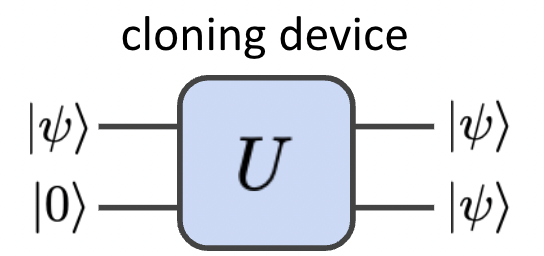
\includegraphics[width=0.8\textwidth]{lesson8/cloning-device.png}
        \caption{A hypothetical cloning device would have to create an unentangled copy of the input state $\ket{\psi}$ on the second qubit initialized in $\ket{0}$.}
    \label{fig:cloner}
\end{figure}

For example if we start in the state $\ket{0}\ket{0}$, after applying our cloning unitary we would like to obtain state $\ket{0}\ket{0}$. That makes sense. If we start in the state $\ket{+}\ket{0}$ and apply our cloning unitary, we would like to obtain as output states, plus for the first qubit and plus for the second qubit, or $\ket{+}\ket{+}$, and so on and so forth until it works for a general input state.

Before we present a proof of what's going on, let's consider some examples to get some intuition.

As a first guess for what our unitary $U$ might be, let's consider a CNOT gate. A CNOT gate represented in the Dirac notation and in the matrix notation is
\begin{equation}
\begin{aligned}
\operatorname{CNOT} &=|0\rangle\langle 0|\otimes I+| 1\rangle\langle 1| \otimes X \\
&=\left(\begin{array}{llll}
1 & 0 & 0 & 0 \\
0 & 1 & 0 & 0 \\
0 & 0 & 0 & 1 \\
0 & 0 & 1 & 0
\end{array}\right)
\end{aligned}
\end{equation}
This means that if the state of the first qubit is zero, then apply the identity to the second qubit, meaning "don't do anything". If the state of the first qubit is one, then apply Pauli $X$ to the second qubit.

Let's consider some inputs and their results,
\begin{equation}
\begin{aligned}
\operatorname{CNOT} |0\rangle|0\rangle &=|0\rangle|0\rangle \\
\operatorname{CNOT} |1\rangle|0\rangle &=|1\rangle|1\rangle \\
\operatorname{CNOT} |+\rangle|0\rangle &=\frac{1}{\sqrt{2}}(|00\rangle+|11\rangle) \\
& \neq|+\rangle|+\rangle
\end{aligned}
\end{equation}
First, let's try a very simple input, $\ket{0}\ket{0}$, as in the first equation above. If we apply CNOT, you can check for yourself that the output is also $\ket{0}\ket{0}$. In this case, we can say that we have cloned the qubit even though we haven't really done anything. The second case is more interesting. We start in the state $\ket{1}\ket{0}$. Now we are trying to clone the state $\ket{1}$, and if the state of the first qubit is one, then we apply the Pauli $X$ to the second qubit.  In fact, our input state is in $\ket{1}$ and our second state is a $\ket{0}$, but after application of the Pauli $X$ it flips into $\ket{1}$. We went from input $\ket{1}\ket{0}$ to output $\ket{1}\ket{1}$. Again, we have cloned our state.

How about if we consider a superposition of zero and one as our input? Our total input is $\ket{+}\ket{0}$. In this case, if you apply the unitary CNOT, you will see that you obtain an entangled state $\ket{0}\ket{0}+\ket{1}\ket{1}$, which is not the product state that we were aiming for. We were aiming for $\ket{+}\ket{+}$. So in this case cloning has failed, at least with this example of CNOT and this particular input.

Let's look at the cases when it worked and then when it didn't. It worked when we were trying to clone the state $\ket{0}$ and the state $\ket{1}$, but it failed when we were trying to clone some superposition of these two states. So it appears that we can only clone states which are orthogonal. Let's try and prove this interesting hypothesis.

Let's say that we are trying to clone an arbitrary state $\ket{\psi}$, so our desired output is $\ket{\psi}\ket{\psi}$.

Let's assume that it works for any two input states. It doesn't matter if our input is $\ket{\psi}$ or some other general state $\ket{\phi}$. We require from our cloning device that it works in any scenario. In the first case when our input set is $\ket{\psi}$, our output is $\ket{\psi} \ket{\psi}$, whereas in the second case when our input is $\ket{\phi}$, our output is $\ket{\phi}\ket{\phi}$,
\begin{equation}
\begin{aligned}
U(\ket{\psi}\ket{0}) &=\ket{\psi}\ket{\psi} \\
U(\ket{\phi}\ket{0}) &=\ket{\phi}\ket{\phi}
\end{aligned}
\end{equation}
Now we can take these two expressions and we can take the inner product of the left hand sides and the right hand sides of these two expressions,
\begin{equation}
\begin{aligned}
(U(\ket{\phi}\ket{0}))^{\dagger}U(\ket{\psi}\ket{0}) &= \bra{\phi}\braket{\phi}{\psi}\ket{\psi} \\
(\bra{0}\bra{\phi}))U^{\dagger}U(\ket{\psi}\ket{0}) &= \braket{\phi}{\psi}\braket{\phi}{\psi} \\
\bra{0}\braket{\phi}{\psi}\ket{0} &= \braket{\phi}{\psi}^2\\
\braket{\phi}{\psi}\braket{0}{0} &= \braket{\phi}{\psi}^2\\
\braket{\phi}{\psi} &= \braket{\phi}{\psi}^2
\end{aligned}
\end{equation}
The right hand side of the equations is quite simple. We take the inner product of $\ket{\phi}$ of the first qubit with $\ket{\psi}$ of the first qubit. To take the inner product, we have to change \ket{\phi} into \bra{\phi}, giving us $\braket{\phi}{\psi}$ in the middle of the equation. That inner product is a scalar (just a number), so we are allowed to move it to the left of the other \ket{\phi}, so we see that we also have the inner product of the second $\ket{\phi}$ and the second $\ket{\psi}$, giving us the value $\braket{\phi}{\psi}^2$. On the left hand side of the two equations, we have the states modified by the unitary operations $U$.  When we take the inner product, the second unitary turns into a $U^\dagger$, and we know that one of the defining properties of a unitary is that $U^\dagger U = I$. So, those unitaries cancel, and what we get is the inner product of $\ket{\phi}$ and $\ket{\psi}$, multiplied by the inner product $\braket{0}{0}$. We know that the inner product $\braket{0}{0} = 1$, so that just cancels out.

On the left hand side, we end up with just the inner product of $\ket{\phi}$ and $\ket{\psi}$, and that has to be equal to the same inner product squared. Now we can easily solve for what the inner product between these two arbitrary states should be. For any scalar $x$, if we have $x = x^2$, then in order to satisfy this equation, $x$ has to be 0 or 1. So what does this actually mean? When the inner product of two states is one, it means that the two states are actually identical, and mathematically we get an identity statement that doesn't tell us anything. On the other hand, when the inner product is zero, it means that the two states are orthogonal.

This proves that our cloning really works, as we saw in the example before, for states that can be distinguished with certainty -- there is no ambiguity or overlap in their superpositions. (Remember, orthogonal states are always distinguishable deterministically.) So we can say that we cannot clone an arbitrary state in quantum mechanics, which is in stark contrast to classical physics. This is the \emph{no-cloning theorem}.

Now let's ask a second interesting question: is teleportation instantaneous? Does it allow us to communicate faster than the speed of light? In order to answer that question, we have to consider the timeline of events that are going on during our teleportation protocol, as in Fig.~\ref{fig:teleportation-timeline}. We start at time $t_0$, when we initialize our system. At some later time $t_1$, Alice performs her measurement in the Bell basis on the two qubits that she has. Then at some later time $t_2$, Alice sends the outcome of the measurements to Bob, and he receives these outcomes at time $t_3$.

Let's go step by step and consider what is going on with Bob's state. At time $t_0$, we said that Bob's qubit is part of a maximally entangled pair, which means that the reduced density of his qubit is a maximally mixed state,
\begin{equation}
\left|\Phi^{+}\right\rangle_{A_2 B}=\frac{1}{\sqrt{2}}(|00\rangle+|11\rangle) \longrightarrow \rho_B=\frac{1}{2}\ketbra{0}{0} +\frac{1}{2}\ketbra{1}{1}.
\end{equation}
This means that if Bob measures his qubit in the Pauli $Z$ basis, he will get the outcome zero ($+1$ eigenvalue) with probability one half, or the outcome one ($-1$ eigenvalue) with probability one half. In fact, if he measures in any basis, he will get the outcome $+1$ or $-1$ with the same probability, so he's maximally unsure about his own state. That also means that he has no idea what state Alice is trying to send him.
\begin{figure}[H]
    \centering
    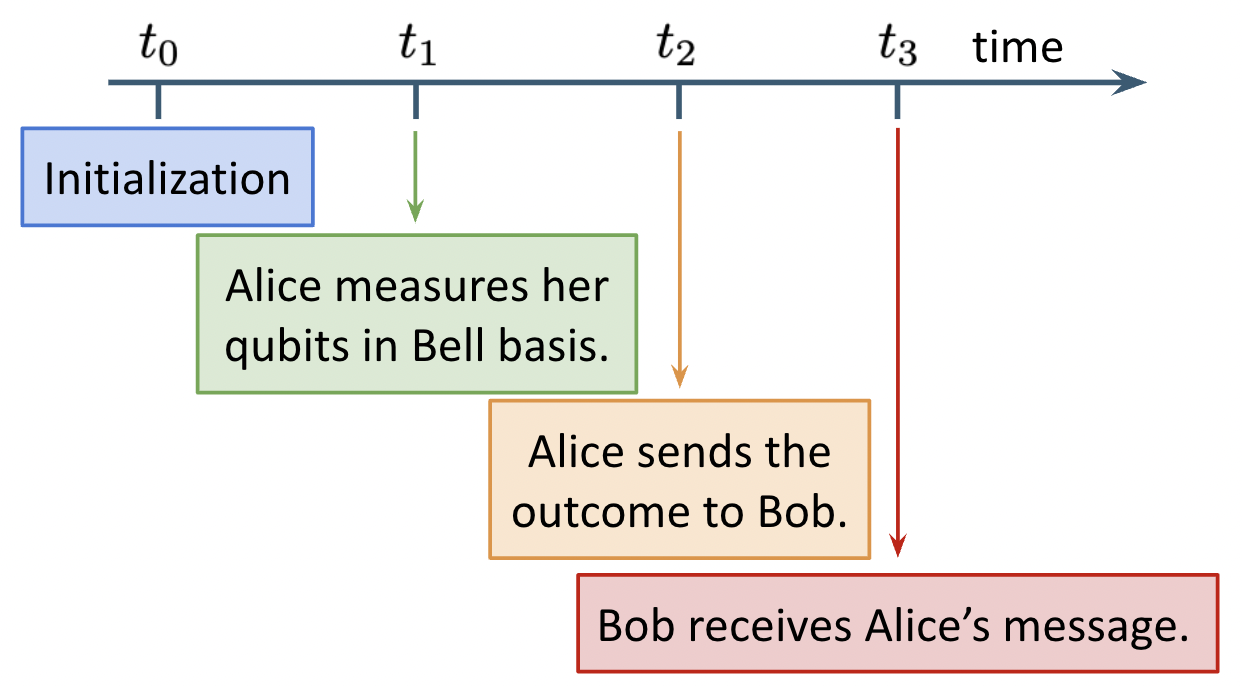
\includegraphics[width=0.8\textwidth]{lesson8/teleportation-timeline.png}
        \caption{The timeline of necessary events and messages in teleportation makes it clear that the speed of light is not violated.}
    \label{fig:teleportation-timeline}
\end{figure}

At time $t_1$, Alice performs her measurement. Just before the measurement, the total state of all three qubits is given by the expression in Eq.~\ref{eq:teleport-alice-basis}. We can rewrite the initial state in terms of the Bell basis for Alice's qubits, which leaves Bob's qubit in the following states subscripted with $B$, depending on which state Alice has. At this time does Bob know anything about Alice's state $A_1$? He doesn't, because nothing really happened. We have only rewritten the initial state.

Then we ask what happens just after $t_1$, just after Alice measures in the Bell basis. Just after the measurement, Bob knows that with probability one quarter, Alice measured the outcome $\ket{\Phi^+}$, and with the same probability she could have obtained each of the other three  Bell states. So he knows that with probability $1/4$, he has the state $\ket{\psi}$, or with probability $1/4$ he has some equivalent state given by these following expressions,\\
$\operatorname{Prob}\left(\left|\Phi^{+}\right\rangle\right)=1 / 4, \quad$ Bob has $\alpha|0\rangle+\beta|1\rangle$\\
$\operatorname{Prob}\left(\left|\Phi^{-}\right\rangle\right)=1 / 4, \quad$ Bob has $\alpha|0\rangle-\beta|1\rangle$\\
$\operatorname{Prob}\left(\left|\Psi^{+}\right\rangle\right)=1 / 4, \quad$ Bob has $\alpha|1\rangle+\beta|0\rangle$\\
$\operatorname{Prob}\left(\left|\Psi^{-}\right\rangle\right)=1 / 4, \quad$ Bob has $\alpha|1\rangle-\beta|0\rangle$.\\

This is a distribution which we can write in the density matrix formalism, so let's do that. Bob's qubit can be written as follows:
\begin{equation}
\begin{aligned}
\rho_B &=\frac{1}{4}(\alpha|0\rangle+\beta|1\rangle)\left(\alpha^*\langle 0|+\beta^*\langle 1|\right) \\
&+\frac{1}{4}(\alpha|0\rangle-\beta|1\rangle)\left(\alpha^*\langle 0|-\beta^*\langle 1|\right) \\
&+\frac{1}{4}(\alpha|1\rangle+\beta|0\rangle)\left(\alpha^*\langle 1|+\beta^*\langle 0|\right) \\
&+\frac{1}{4}(\alpha|1\rangle-\beta|0\rangle)\left(\alpha^*\langle 1|-\beta^*\langle 0|\right) \\
&=\frac{1}{2}\left(|\alpha|^2+|\beta|^2\right)\ketbra{0}{0} \\
&+\frac{1}{2}\left(|\alpha|^2+|\beta|^2\right)\ketbra{1}{1} \\
&=\frac{1}{2}\ketbra{0}{0}+\frac{1}{2}\ketbra{1}{1}
\end{aligned}
\end{equation}
%with probability a quarter, he has the state alpha zero plus beta one, which in density matrix formalism is given by the outer product. With probability one quarter, here's the following state, and so on and so forth for the other two possibilities. 
We can go through the algebra and we will see that the cross terms cancel, and in fact what we obtain is that the state of Bob, given by $\rho_B$, which can simplify to, again, a maximally mixed state. This is because we started with state $\ket{\psi}$ which is normalized, meaning $|\alpha|^2+|\beta|^2 = 1$. So even just after the measurement, Bob still doesn't know anything about the state $\ket{\psi}$. His qubit is maximally mixed.

Let's see what happens when we go to time $t_2$. At this time, we say that Alice sends the outcome to Bob. Well, nothing really changes from just after the measurement occurred at time $t_1$, because Bob has not received the message about the outcomes of the measurements, so his state is still the maximally mixed state. He has no information about the state to be teleported, $\ket{\psi}$. So teleportation still has not been completed, even though the measurement by Alice has been performed at time $t_1$. Finally, at time $t_3$, Bob receives Alice's message containing two classical bits telling him about which outcome she measured.

Bob finally has the following state: he has the state $\ket{\psi}$ up to some unitary, Pauli $X$, $Y$, or the product of $X$ and $Y$. So it's only at time $t_3$, when he receives the message, that teleportation really, truly, has taken place. Bob must receive the classical message in order for teleportation to work, so he has to wait all this time from $t_2$ to $t_3$ to receive this message, which can travel at best at the speed of light. So we don't communicate faster than the speed of light and we do not violate special relativity.


\section{Simulating teleportation}
\label{sec:8-4_simulating}

(Hands-on exercises for simulating teleportation to be added as a Jupyter Qiskit notebook.)


\newpage
\begin{exercises}

\exer{Return to the exercises on measurement in Ch.~\ref{sec:2_quantum_states}. Let's do the math on teleportation using the notation of Ex.~\ref{ex:dirac-notation-measurement}. \rdv{Label numbering seems busted.}
\subexer{
For measuring two qubits together, we need four measurement operators.
Write out the measurement operators in the computational basis using the Dirac notation and for the full matrix notation.
}
\subexer{
Find the Bell basis measurement operators for two qubits. Write them out in both the Dirac notation and the full matrix notation.
}
\rdv{More on the math of projections and traces using the full measurement equation and on measuring subsets of qubits in multi-qubit states.}
}

\end{exercises}

